\documentclass[11pt,letterpaper]{article}

\usepackage[margin=1in]{geometry}
\usepackage{graphicx}
\usepackage{amsmath,amssymb}
\usepackage{booktabs}
\usepackage{longtable}
\usepackage{listings}
\usepackage{xcolor}
\usepackage{hyperref}
\usepackage{tikz}
\usetikzlibrary{arrows.meta,positioning,shapes.geometric,fit,calc}
\usepackage{bytefield}
\usepackage{fancyhdr}
\usepackage{titlesec}
\usepackage{enumitem}
\usepackage{caption}

% Brand colors
\definecolor{garnet}{HTML}{73000A}
\definecolor{black90}{HTML}{363636}
\definecolor{black70}{HTML}{5C5C5C}
\definecolor{black50}{HTML}{A2A2A2}
\definecolor{black30}{HTML}{C7C7C7}
\definecolor{black10}{HTML}{ECECEC}
\definecolor{atlantic}{HTML}{466A9F}
\definecolor{congaree}{HTML}{1F414D}
\definecolor{horseshoe}{HTML}{65780B}
\definecolor{rose}{HTML}{CC2E40}
\definecolor{honeycomb}{HTML}{A49137}

\hypersetup{
    colorlinks=true,
    linkcolor=garnet,
    urlcolor=atlantic,
    citecolor=congaree,
}

\lstset{
    basicstyle=\ttfamily\small,
    keywordstyle=\color{garnet}\bfseries,
    commentstyle=\color{black50},
    stringstyle=\color{atlantic},
    frame=single,
    framerule=0.5pt,
    rulecolor=\color{black30},
    backgroundcolor=\color{black10},
    breaklines=true,
    showstringspaces=false,
    tabsize=4,
    xleftmargin=1em,
    xrightmargin=1em,
}

\pagestyle{fancy}
\fancyhf{}
\fancyhead[L]{\textcolor{garnet}{\textsc{Furuno DRS4DL+ Technical Manual}}}
\fancyhead[R]{\textcolor{black70}{\thepage}}
\fancyfoot[C]{\textcolor{black50}{\small J.C. Vaught --- University of South Carolina}}
\renewcommand{\headrulewidth}{0.5pt}
\renewcommand{\headrule}{\hbox to\headwidth{\color{garnet}\leaders\hrule height \headrulewidth\hfill}}

\titleformat{\section}{\Large\bfseries\color{garnet}}{}{0em}{}
\titleformat{\subsection}{\large\bfseries\color{congaree}}{}{0em}{}
\titleformat{\subsubsection}{\normalsize\bfseries\color{black90}}{}{0em}{}

\title{
    \vspace{-1cm}
    {\color{garnet}\rule{\textwidth}{2pt}}\\[0.5cm]
    {\Huge\bfseries\color{garnet} Furuno DRS4DL+ Radar}\\[0.3cm]
    {\LARGE\color{black90} Wire Protocol \& System Technical Manual}\\[0.3cm]
    {\color{garnet}\rule{\textwidth}{2pt}}
}
\author{J.C. Vaught\\
\texttt{jvaught@sc.edu}\\[0.3em]
University of South Carolina}
\date{March 2026}

\begin{document}
\maketitle
\thispagestyle{fancy}
\tableofcontents
\newpage

%=============================================================================
\section{Introduction}
%=============================================================================

This document provides a comprehensive technical reference for the Furuno DRS4DL+ marine radar system as interfaced through the \texttt{radar-client} Rust application. It covers the complete wire protocol, echo data encoding, system architecture, web API, and calibration procedures. All information was obtained through reverse engineering of the proprietary \texttt{libNAVNETDLL.so} shared library and live packet captures from the radar hardware.

The Furuno DRS4DL+ is a solid-state Doppler radar operating in the X-band (9.41~GHz). It communicates with its host processor over Ethernet using a combination of TCP control channels and UDP multicast for echo data delivery.

\subsection{Hardware Overview}

The radar unit (scanner) contains the antenna, transmitter, and receiver in a single radome enclosure. It connects to the host processor (in this case, a Raspberry Pi) via a standard Ethernet cable. The scanner has a fixed IP address of \texttt{172.31.3.226} on a \texttt{/16} subnet.

\subsection{Software Components}

The system consists of three main software components.

The \textbf{radar-client} is a Rust binary that implements the full Furuno wire protocol. It handles authentication, control commands, echo data reception and decoding, PPI rendering, and serves a web interface for browser-based operation.

The \textbf{web interface} is a set of static HTML/CSS/JavaScript files served by the Rust application. It provides real-time PPI display, radar settings controls, recording capabilities, and pattern-based calibration tools.

The \textbf{protocol-notes} directory contains the original reverse-engineering artifacts: packet captures, symbol tables from the proprietary library, and analysis documents that informed this implementation.


%=============================================================================
\section{Network Architecture}
%=============================================================================

\subsection{Topology}

The radar and host communicate over a dedicated Ethernet link on the \texttt{172.31.0.0/16} subnet. The host may also have additional network interfaces (Wi-Fi, Tailscale VPN) for external access to the web interface.

\begin{figure}[h]
\centering
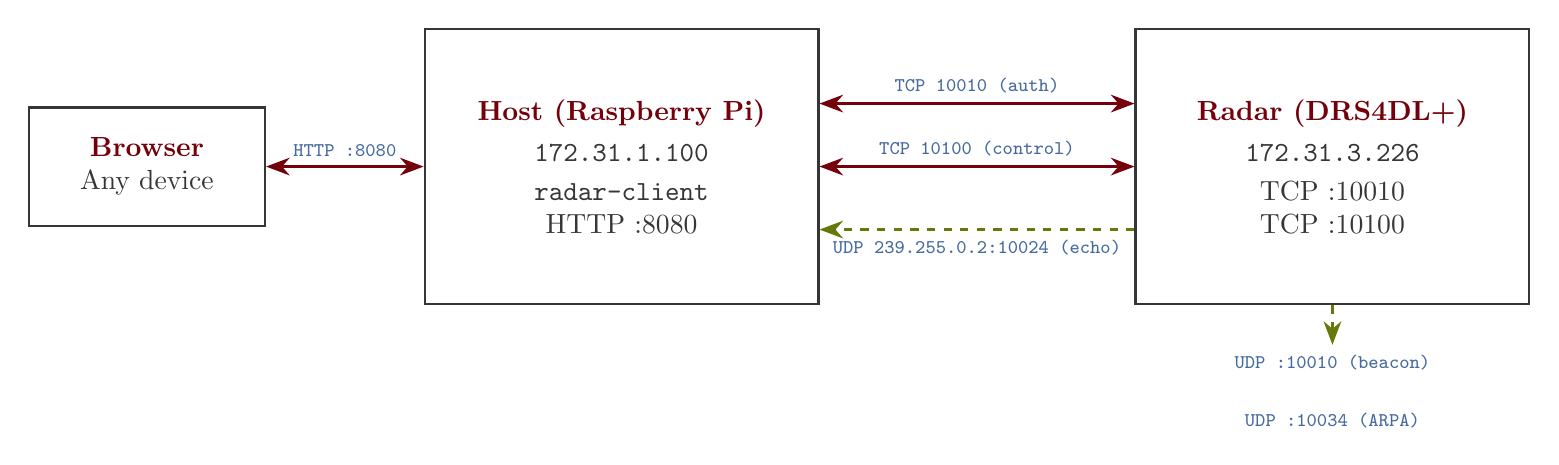
\begin{tikzpicture}[
    node distance=4cm,
    box/.style={draw, thick, minimum width=5cm, minimum height=3.5cm, align=center, color=black90},
    port/.style={font=\ttfamily\scriptsize, color=atlantic},
    arrow/.style={-{Stealth[length=3mm]}, thick, color=garnet},
    biarrow/.style={{Stealth[length=3mm]}-{Stealth[length=3mm]}, thick, color=garnet},
    mcast/.style={-{Stealth[length=3mm]}, thick, dashed, color=horseshoe},
]

% Host box
\node[box] (host) {
    \textbf{\color{garnet}Host (Raspberry Pi)}\\[0.3em]
    \texttt{172.31.1.100}\\[0.2em]
    \texttt{radar-client}\\
    HTTP :8080
};

% Radar box
\node[box, right=4cm of host] (radar) {
    \textbf{\color{garnet}Radar (DRS4DL+)}\\[0.3em]
    \texttt{172.31.3.226}\\[0.2em]
    TCP :10010\\
    TCP :10100
};

% Connection arrows
\draw[biarrow] ([yshift=0.8cm]host.east) -- ([yshift=0.8cm]radar.west)
    node[midway, above, port] {TCP 10010 (auth)};

\draw[biarrow] ([yshift=0cm]host.east) -- ([yshift=0cm]radar.west)
    node[midway, above, port] {TCP 10100 (control)};

\draw[mcast] ([yshift=-0.8cm]radar.west) -- ([yshift=-0.8cm]host.east)
    node[midway, below, port] {UDP 239.255.0.2:10024 (echo)};

% Broadcast below
\node[port, below=0.5cm of radar] (bcast) {UDP :10010 (beacon)};
\draw[mcast] (radar.south) -- (bcast);

\node[port, below=0.3cm of bcast] (arpa) {UDP :10034 (ARPA)};

% Browser
\node[box, minimum height=1.5cm, minimum width=3cm, left=2cm of host] (browser) {
    \textbf{\color{garnet}Browser}\\
    Any device
};
\draw[biarrow] (browser.east) -- (host.west)
    node[midway, above, port] {HTTP :8080};

\end{tikzpicture}
\caption{Network topology of the radar system.}
\label{fig:topology}
\end{figure}


\subsection{Port Map}

Table~\ref{tab:ports} lists all network ports used by the system.

\begin{table}[h]
\centering
\caption{Network port assignments.}
\label{tab:ports}
\begin{tabular}{@{}llllr@{}}
\toprule
\textbf{Port} & \textbf{Direction} & \textbf{Protocol} & \textbf{Purpose} & \textbf{Rate} \\
\midrule
10010 & Host $\leftrightarrow$ Radar & TCP & One-shot authentication & Once \\
10010 & Radar $\to$ Broadcast & UDP & Discovery beacon & $\sim$1/16\,s \\
10024 & Radar $\to$ 239.255.0.2 & UDP & Echo sweep data & $\sim$80/s \\
10034 & Radar $\to$ Broadcast & UDP & ARPA target data & $\sim$1/s \\
10100 & Host $\leftrightarrow$ Radar & TCP & Persistent control channel & $\sim$2/s \\
8080 & Browser $\leftrightarrow$ Host & HTTP & Web interface & On demand \\
\bottomrule
\end{tabular}
\end{table}


\subsection{Auto-Discovery and Network Configuration}

The radar broadcasts a UDP beacon on port 10010 approximately every 16 seconds. The \texttt{radar-client} application uses this beacon for auto-discovery. On startup, the client broadcasts probe packets on all detected network interfaces and listens for radar responses.

If the host has no interface on the radar's subnet, the application automatically adds a secondary IP alias to the physical Ethernet interface. This is handled in a platform-specific manner: \texttt{ip addr add} on Linux, \texttt{ifconfig alias} on macOS, and \texttt{netsh interface ip add address} on Windows.

The discovery process follows three stages. First, the client checks for explicit \texttt{--radar-ip} and \texttt{--host-ip} command-line flags. Second, if no flags are provided, it broadcasts UDP beacons on all interfaces for 3 seconds. Third, if discovery fails, it falls back to the default addresses (\texttt{172.31.3.226} and \texttt{172.31.1.100}) and ensures subnet reachability via auto-alias.


%=============================================================================
\section{Control Protocol}
%=============================================================================

The radar uses an NMEA-like ASCII protocol over TCP port 10100 for all control and status communication. A separate one-shot TCP connection on port 10010 handles initial authentication.

\subsection{Message Format}

All control messages follow the general format:

\begin{lstlisting}
$<prefix><hex_id>,<param1>,<param2>,...\r\n
\end{lstlisting}

Three message prefixes are defined in Table~\ref{tab:prefixes}.

\begin{table}[h]
\centering
\caption{Control message prefixes.}
\label{tab:prefixes}
\begin{tabular}{@{}lll@{}}
\toprule
\textbf{Prefix} & \textbf{Direction} & \textbf{Meaning} \\
\midrule
\texttt{\$S} & Host $\to$ Radar & Set/Send command \\
\texttt{\$R} & Host $\to$ Radar & Read/Request register \\
\texttt{\$N} & Radar $\to$ Host & Notify/Acknowledge response \\
\bottomrule
\end{tabular}
\end{table}

Command IDs are two-character hexadecimal values (e.g., \texttt{62} for range, \texttt{69} for TX state). Parameters are comma-separated decimal integers. Messages are terminated with \texttt{\textbackslash r\textbackslash n} (0x0D 0x0A).

\subsection{Binary Keepalive}

In addition to ASCII messages, the control channel uses an 8-byte binary keepalive packet sent every 5--10 seconds.

\begin{figure}[h]
\centering
\begin{bytefield}[bitwidth=1.5em]{32}
\bitheader{0-31} \\
\bitbox{32}{\texttt{00 00 00 08}} \\
\bitbox{32}{\texttt{00 00 00 00}}
\end{bytefield}
\caption{Binary keepalive packet (8 bytes). The first 4 bytes encode the packet length.}
\label{fig:keepalive}
\end{figure}

The keepalive must be distinguished from ASCII messages by checking the first byte: if byte 0 is \texttt{0x00} and the total length is 8, the packet is a keepalive rather than an ASCII command.

\subsection{Initialization Sequence}

The full cold-start initialization proceeds through six phases, illustrated in Figure~\ref{fig:init_sequence}.

\begin{figure}[h]
\centering
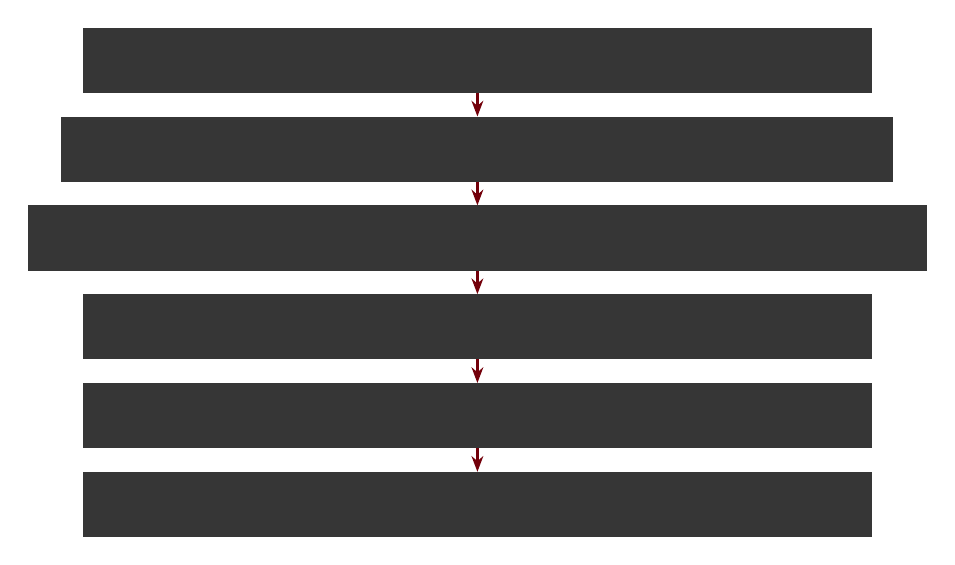
\begin{tikzpicture}[
    phase/.style={draw, thick, minimum width=10cm, minimum height=0.8cm, align=center, fill=black10, color=black90},
    arrow/.style={-{Stealth[length=2mm]}, thick, color=garnet},
    note/.style={font=\small\itshape, color=black70},
]

\node[phase] (p1) at (0,0) {\textbf{Phase 1:} Radar broadcasts beacon on UDP 10010};
\node[phase, below=0.3cm of p1] (p2) {\textbf{Phase 2:} TCP 10010 authentication (56-byte copyright exchange)};
\node[phase, below=0.3cm of p2] (p3) {\textbf{Phase 3:} TCP 10100 control channel open $\to$ \texttt{\$N00,CLIENTCONNECTION}};
\node[phase, below=0.3cm of p3] (p4) {\textbf{Phase 4:} Firmware query (\texttt{\$R96}) $\to$ version strings};
\node[phase, below=0.3cm of p4] (p5) {\textbf{Phase 5:} Bulk register reads (184 \texttt{\$R} commands)};
\node[phase, below=0.3cm of p5] (p6) {\textbf{Phase 6:} Ready for TX ON and echo data};

\foreach \i/\j in {p1/p2, p2/p3, p3/p4, p4/p5, p5/p6} {
    \draw[arrow] (\i.south) -- (\j.north);
}

\end{tikzpicture}
\caption{Initialization sequence phases.}
\label{fig:init_sequence}
\end{figure}


\subsubsection{Phase 1: Discovery}

The radar continuously broadcasts a 32-byte discovery beacon on UDP port 10010 to the subnet broadcast address (\texttt{172.31.255.255}). The beacon contains the device identifier (e.g., ``RD003226'') at byte offset 16.

\begin{lstlisting}
01 00 00 01 00 00 00 00   (header)
00 01 00 18 01 00 00 00   (capability/type)
52 44 30 30 33 32 32 36   ("RD003226")
01 01 00 02 00 01 00 12   (device type/version)
\end{lstlisting}

\subsubsection{Phase 2: Authentication}

The host opens a TCP connection to the radar on port 10010 and sends a 56-byte binary payload containing a Furuno copyright string. The radar responds with a 12-byte acknowledgment.

\begin{lstlisting}
Host sends (56 bytes):
  08 01 00 38 01 00 00 00 00 01 00 00
  COPYRIGHT (C) 2001 FURUNO ELECTRIC CO.,LTD.

Radar responds (12 bytes):
  09 01 00 0C 01 00 00 00 00 64 00 00
\end{lstlisting}

Authentication succeeds when byte 9 of the response equals \texttt{0x64} (decimal 100). The TCP connection is closed immediately after this exchange.

\subsubsection{Phase 3: Control Channel}

The host opens a persistent TCP connection to port 10100 with \texttt{TCP\_NODELAY} enabled. The radar immediately sends a connection confirmation.

\begin{lstlisting}
$N00,CLIENTCONNECTION,\r\n
\end{lstlisting}

\subsubsection{Phase 4: Firmware Query}

The host sends a firmware version request.

\begin{lstlisting}
$R96,,,,,,,\r\n
\end{lstlisting}

The radar responds with firmware version strings for each subsystem.

\begin{lstlisting}
$N96,0359360-01.07,0359358-01.01,0359359-01.02,0359361-01.06,,,
\end{lstlisting}


\subsubsection{Phase 5: Register Dump}

The host sends approximately 184 register read commands (\texttt{\$R}) in rapid succession, covering register IDs from \texttt{0x61} through \texttt{0xFD}. The radar responds to each with a \texttt{\$N} notification containing the current register values. This establishes the initial state of all radar parameters.

\subsubsection{Phase 6: Steady State}

After initialization, the control channel enters steady state. The radar periodically sends antenna heading reports (\texttt{\$NAF,256}) at approximately 1\,Hz and binary keepalive packets every 5--10 seconds. No echo data is transmitted until TX is explicitly enabled.


%=============================================================================
\section{Command Reference}
%=============================================================================

This section documents all implemented control commands. Each command is sent as an ASCII \texttt{\$S} message on the TCP 10100 control channel.

\subsection{TX State (\texttt{\$S69})}

Controls the radar transmitter power state.

\begin{lstlisting}
$S69,<state>,0,0,0,0,0\r\n
\end{lstlisting}

The \texttt{state} parameter is 1 for TX OFF (standby) and 2 for TX ON. Note the counterintuitive assignment where 2 enables transmission.

A TX toggle is always accompanied by three auxiliary commands sent atomically within approximately 1\,ms.

\begin{lstlisting}
$S69,2,0,0,0,0,0    (TX ON)
$S85,0               (A/C SEA reset)
$S86,0               (A/C SEA mode reset)
$S87,0               (A/C RAIN reset)
\end{lstlisting}


\subsection{Range (\texttt{\$S62})}

Sets the radar display range.

\begin{lstlisting}
$S62,<wireIndex>,0,0,0\r\n
\end{lstlisting}

Table~\ref{tab:ranges} maps wire indices to physical distances.

\begin{table}[h]
\centering
\caption{Range wire index mapping.}
\label{tab:ranges}
\begin{tabular}{@{}rrr@{}}
\toprule
\textbf{Wire Index} & \textbf{Meters} & \textbf{Label} \\
\midrule
21 & 116 & 1/16 NM \\
0 & 231 & 1/8 NM \\
1 & 463 & 1/4 NM \\
2 & 926 & 1/2 NM \\
3 & 1{,}389 & 3/4 NM \\
4 & 1{,}852 & 1 NM \\
5 & 2{,}778 & 1.5 NM \\
6 & 3{,}704 & 2 NM \\
7 & 5{,}556 & 3 NM \\
8 & 7{,}408 & 4 NM \\
9 & 11{,}112 & 6 NM \\
10 & 14{,}816 & 8 NM \\
11 & 22{,}224 & 12 NM \\
12 & 29{,}632 & 16 NM \\
13 & 44{,}448 & 24 NM \\
14 & 59{,}264 & 32 NM \\
19 & 66{,}672 & 36 NM \\
15 & 88{,}896 & 48 NM \\
\bottomrule
\end{tabular}
\end{table}


\subsection{Gain (\texttt{\$S63})}

Controls radar receiver gain.

\begin{lstlisting}
$S63,<channel>,<value>,0,<maxGain>,0\r\n
\end{lstlisting}

The \texttt{channel} parameter selects between manual gain (0) and auto gain (1). For manual mode, the \texttt{value} parameter ranges from 0 to 255.


\subsection{Sea Clutter (\texttt{\$S85}/\texttt{\$S86})}

Controls the A/C SEA (anti-clutter sea) filter.

\begin{lstlisting}
$S85,<value>\r\n     (A/C SEA level, 0-255)
$S86,<value>\r\n     (A/C SEA mode)
\end{lstlisting}


\subsection{Rain Clutter (\texttt{\$S87})}

Controls the A/C RAIN (anti-clutter rain) filter.

\begin{lstlisting}
$S87,<value>\r\n     (A/C RAIN level, 0-255)
\end{lstlisting}


\subsection{Pulse Width (\texttt{\$S65})}

Sets the transmitter pulse width.

\begin{lstlisting}
$S65,<channel>,<value>,0,0,0,0,0\r\n
\end{lstlisting}

The \texttt{value} parameter ranges from 0 to 3, where 0 is the shortest pulse and 3 is the longest.


\subsection{STC --- Sensitivity Time Control (\texttt{\$S64})}

Controls the near, middle, and far STC curves. The \texttt{channel} parameter selects the STC region.

\begin{lstlisting}
$S64,<channel>,<value>,0,0,0,0\r\n
\end{lstlisting}

There are three STC regions: near (\texttt{channel}=0), middle (\texttt{channel}=1), and far (\texttt{channel}=2). Dedicated convenience commands also exist for individual STC regions.

\begin{lstlisting}
$S85,<value>\r\n     (near STC)
$S86,<value>\r\n     (middle STC)
$S87,<value>\r\n     (far STC)
\end{lstlisting}


\subsection{Main Bang Suppression (\texttt{\$S83})}

Suppresses the main bang (transmitter pulse leakage) at close range.

\begin{lstlisting}
$S83,<value>,0\r\n
\end{lstlisting}


\subsection{Bearing Resolution / Rez Boost (\texttt{\$SEE})}

Controls the bearing resolution enhancement.

\begin{lstlisting}
$SEE,<level>,0\r\n
\end{lstlisting}

The \texttt{level} parameter takes values 0 (off), 1 (low), 2 (medium), or 3 (high). Rez boost affects the ratio of short to long pulse types in the dual-pulse echo data (see Section~\ref{sec:dualpulse}).


\subsection{Interference Rejection (\texttt{\$S88})}

Controls the interference rejection filter.

\begin{lstlisting}
$S88,<enabled>\r\n
\end{lstlisting}

The \texttt{enabled} parameter is 0 for off and 1 for on.


\subsection{Bird Mode (\texttt{\$SBD})}

Controls bird echo suppression.

\begin{lstlisting}
$SBD,<level>\r\n
\end{lstlisting}

The \texttt{level} parameter ranges from 0 (off) to 3 (maximum suppression).


\subsection{Antenna Revolution Speed (\texttt{\$S89})}

Controls the antenna rotation speed.

\begin{lstlisting}
$S89,<speed>,<hiRpm>\r\n
\end{lstlisting}

The \texttt{speed} parameter selects the rotation mode. The \texttt{hiRpm} flag enables high-speed operation.


\subsection{Doppler / Echo Color Type (\texttt{\$SEF})}

Controls the Doppler target analyzer mode.

\begin{lstlisting}
$SEF,<mode>,<sw>,<autoPicture>,0\r\n
\end{lstlisting}

The \texttt{mode} parameter takes values 0 (off), 1 (Target Analyzer), or 2 (alternative mode). The \texttt{sw} parameter enables (1) or disables (0) the feature. See Section~\ref{sec:doppler} for details on how Doppler information is encoded in echo data.


\subsection{Antenna Height (\texttt{\$S82})}

Sets the antenna installation height above sea level.

\begin{lstlisting}
$S82,<meters>,0,0,0,0\r\n
\end{lstlisting}


\subsection{No-Transmit Sectors (\texttt{\$S67})}

Defines angular sectors where the transmitter is inhibited.

\begin{lstlisting}
$S67,<startAngle>,<endAngle>,<sectorIndex>,0\r\n
\end{lstlisting}

Up to 32 no-transmit sectors can be defined (sector indices 0--31). Angles are specified in tenths of a degree (0--3599).


\subsection{Noise Reduction (\texttt{\$S8A})}

Controls the echo noise reduction filter.

\begin{lstlisting}
$S8A,<enabled>\r\n
\end{lstlisting}


\subsection{Scan Speed (\texttt{\$S8C})}

Controls the scan processing speed.

\begin{lstlisting}
$S8C,<mode>\r\n
\end{lstlisting}


%=============================================================================
\section{Periodic Telemetry}
%=============================================================================

The radar sends unsolicited \texttt{\$N} notifications on the control channel at regular intervals. Table~\ref{tab:telemetry} lists the observed periodic messages.

\begin{table}[h]
\centering
\caption{Periodic telemetry messages.}
\label{tab:telemetry}
\begin{tabular}{@{}llp{7cm}@{}}
\toprule
\textbf{Message} & \textbf{Rate} & \textbf{Content} \\
\midrule
\texttt{\$NAF,256} & $\sim$1/s & Antenna heading/rotation indicator \\
\texttt{\$NF5,\ldots} & $\sim$1/s & Radar spoke/scan telemetry \\
\texttt{\$NE0,\ldots} & Periodic & Extended status (8 fields) \\
\texttt{\$N83,100,1} & Periodic & Gain/threshold report \\
\texttt{\$N68,\ldots} & Periodic & Status with negative values \\
\texttt{\$N00,CLIENTCONNECTION} & Once & Connection established notification \\
\texttt{[keepalive]} & 5--10\,s & 8-byte binary keepalive \\
\bottomrule
\end{tabular}
\end{table}


%=============================================================================
\section{Echo Data Format}
%=============================================================================

Echo data arrives via UDP multicast on address \texttt{239.255.0.2}, port 10024. Packets arrive at approximately 80 per second ($\sim$12\,ms interval) and contain one or more radar spokes (radial sweep lines).

\subsection{Packet Structure}

Each UDP echo packet consists of a 16-byte header followed by one or more spoke payloads.

\begin{figure}[h]
\centering
\begin{bytefield}[bitwidth=0.85em]{32}
\bitheader{0,7,8,15,16,23,24,31} \\
\begin{rightwordgroup}{Header\\(16 bytes)}
\bitbox{16}{Sequence/Spoke Counter} & \bitbox{16}{Protocol Version (\texttt{0x0001})} \\
\bitbox{32}{Reserved (\texttt{0x00000000})} \\
\bitbox{32}{Timestamp} \\
\bitbox{16}{Flags (\texttt{0x1500})} & \bitbox{16}{Config (\texttt{0xF009})}
\end{rightwordgroup} \\
\begin{rightwordgroup}{Spoke $n$}
\bitbox{16}{Azimuth Angle (ticks)} & \bitbox{16}{Heading (ticks)} \\
\bitbox{32}{Encoded Echo Data (variable length)\ldots}
\end{rightwordgroup}
\end{bytefield}
\caption{Echo UDP packet layout.}
\label{fig:echo_packet}
\end{figure}


\subsection{Echo Metadata}

Key metadata is extracted from the 16-byte header. The sweep count (number of spokes in the packet) is derived from byte 9, bit-shifted right by 1. The sweep length (number of range bins per spoke) is encoded across bytes 10--11. The encoding type occupies bits 4:3 of byte 11.

\begin{align}
\texttt{sweep\_count} &= \texttt{data[9]} \gg 1 \\
\texttt{sweep\_len} &= ((\texttt{data[11]} \mathbin{\&} \texttt{0x07}) \ll 8) \mathbin{|} \texttt{data[10]} \\
\texttt{encoding} &= (\texttt{data[11]} \mathbin{\&} \texttt{0x18}) \gg 3
\end{align}


\subsection{Azimuth and Heading}

Each spoke begins with a 4-byte sub-header containing the azimuth angle and heading in 16-bit little-endian tick values. The radar uses 8{,}192 ticks per full rotation ($360\degree$).

\begin{equation}
\theta_{\text{deg}} = \frac{\texttt{angle\_ticks}}{8192} \times 360\degree
\end{equation}

The heading field tracks the antenna's compass bearing independently of the spoke azimuth.


\subsection{Echo Encoding Types}
\label{sec:encoding}

The radar uses four encoding schemes for echo amplitude data, selected by the encoding field in the packet header. All encodings produce a fixed-length array of range bins (typically 868 bins). After decoding, wire values are right-shifted by 2 bits for display: $\texttt{display} = \texttt{wire} \gg 2$.

\subsubsection{Encoding 0: Raw Uncompressed}

Echo bytes are stored directly with no compression. The decoded spoke is simply the first \texttt{sweep\_len} bytes of the payload, zero-padded if necessary. Consumed bytes are rounded up to a 4-byte boundary.

\subsubsection{Encoding 1: RLE with Repeat Marker}

Uses single-byte run-length encoding. The least significant bit (LSB) distinguishes literal values from repeat markers.

If $\texttt{LSB} = 0$, the byte is a literal echo amplitude value. If $\texttt{LSB} = 1$, the byte encodes a repeat count for the previous amplitude value: $\texttt{count} = \texttt{byte} \gg 1$, with a count of 0 meaning 128 repeats.

\subsubsection{Encoding 2: Delta RLE with Previous Spoke Reference}

Similar to Encoding 1, but repeat markers copy from the \textit{previous spoke} at the corresponding range bin index rather than repeating the last literal value. The first spoke in a packet uses Encoding 1 since no previous spoke reference is available.

\subsubsection{Encoding 3: 2-Bit RLE with Dual Reference}

Uses the two least significant bits for control. If $\texttt{bits}[1{:}0] = 00$, the byte is a literal value. If $\texttt{bit}[0] = 1$, repeat the previous literal value with count $= \texttt{byte} \gg 2$ (0 means 64). If $\texttt{bits}[1{:}0] = 10$, copy from the previous spoke with count $= \texttt{byte} \gg 2$ (0 means 64).

\begin{figure}[h]
\centering
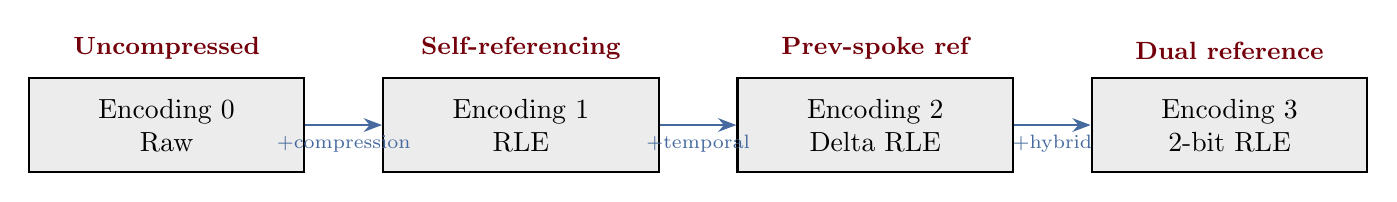
\begin{tikzpicture}[
    enc/.style={draw, thick, minimum width=3.5cm, minimum height=1.2cm, align=center, fill=black10},
    label/.style={font=\small\bfseries, color=garnet},
]
\node[enc] (e0) at (0,0) {Encoding 0\\Raw};
\node[enc] (e1) at (4.5,0) {Encoding 1\\RLE};
\node[enc] (e2) at (9,0) {Encoding 2\\Delta RLE};
\node[enc] (e3) at (13.5,0) {Encoding 3\\2-bit RLE};

\node[label, above=0.1cm of e0] {Uncompressed};
\node[label, above=0.1cm of e1] {Self-referencing};
\node[label, above=0.1cm of e2] {Prev-spoke ref};
\node[label, above=0.1cm of e3] {Dual reference};

\draw[-{Stealth}, thick, color=atlantic] (e0) -- (e1) node[midway, below, font=\scriptsize] {+compression};
\draw[-{Stealth}, thick, color=atlantic] (e1) -- (e2) node[midway, below, font=\scriptsize] {+temporal};
\draw[-{Stealth}, thick, color=atlantic] (e2) -- (e3) node[midway, below, font=\scriptsize] {+hybrid};
\end{tikzpicture}
\caption{Progression of echo encoding complexity.}
\label{fig:encoding_types}
\end{figure}


%=============================================================================
\section{Doppler Processing}
\label{sec:doppler}
%=============================================================================

The DRS4DL+ supports Doppler target analysis, which repurposes the most significant bit of each echo byte to encode target motion information.

\subsection{Status Field Encoding}

The \texttt{status} field in each echo spoke carries the Doppler active flag in bit 8 (0x100).

\begin{table}[h]
\centering
\caption{Status field bit layout.}
\label{tab:status}
\begin{tabular}{@{}rrl@{}}
\toprule
\textbf{Status} & \textbf{Binary} & \textbf{Meaning} \\
\midrule
1 (0x01) & \texttt{0\_0000\_0001} & Normal echo, long pulse (coarse) \\
4 (0x04) & \texttt{0\_0000\_0100} & Normal echo, short pulse (fine) \\
257 (0x101) & \texttt{1\_0000\_0001} & Doppler echo, long pulse \\
260 (0x104) & \texttt{1\_0000\_0100} & Doppler echo, short pulse \\
\bottomrule
\end{tabular}
\end{table}

The confirmed bit layout is as follows. Bit 8 is the Doppler active flag (0 = normal, 1 = Doppler data present in echo bit 7). Bits 2:0 encode the pulse type (1 = long/coarse, 4 = short/fine, interleaved per spoke).

\subsection{Echo Byte Encoding}

When Doppler is \textbf{disabled} (status bit 8 = 0), the full 8-bit range is used for echo intensity (0--252). Approximately 26\% of echo bytes have bit 7 set in normal operation.

When Doppler is \textbf{enabled} (status bit 8 = 1), the echo byte is split. Bit 7 serves as the Doppler direction flag (0 = stationary, 1 = moving target). Bits 6:0 encode echo intensity compressed to 7 bits (0--126).

\begin{figure}[h]
\centering
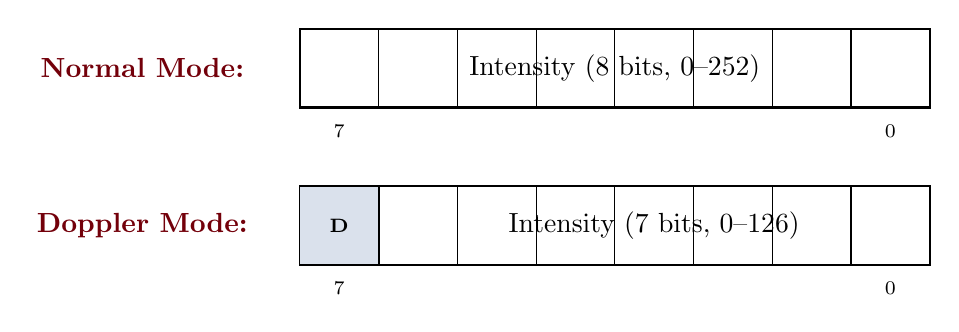
\begin{tikzpicture}
% Normal mode
\node[font=\bfseries\color{garnet}] at (-2, 1.5) {Normal Mode:};
\draw[thick] (0,1) rectangle (8,2);
\foreach \x in {1,...,7} {
    \draw (\x,1) -- (\x,2);
}
\node at (4, 1.5) {Intensity (8 bits, 0--252)};
\node[font=\scriptsize] at (0.5, 0.7) {7};
\node[font=\scriptsize] at (7.5, 0.7) {0};

% Doppler mode
\node[font=\bfseries\color{garnet}] at (-2, -0.5) {Doppler Mode:};
\draw[thick] (0,-1) rectangle (8,0);
\draw[thick] (1,-1) -- (1,0);
\foreach \x in {2,...,7} {
    \draw (\x,-1) -- (\x,0);
}
\draw[fill=atlantic!20] (0,-1) rectangle (1,0);
\node[font=\scriptsize] at (0.5, -0.5) {\textbf{D}};
\node at (4.5, -0.5) {Intensity (7 bits, 0--126)};
\node[font=\scriptsize] at (0.5, -1.3) {7};
\node[font=\scriptsize] at (7.5, -1.3) {0};
\end{tikzpicture}
\caption{Echo byte layout in normal vs. Doppler mode. The D bit indicates a moving target.}
\label{fig:doppler_byte}
\end{figure}


%=============================================================================
\section{Dual-Pulse Interleaving}
\label{sec:dualpulse}
%=============================================================================

The radar alternates between long and short transmitter pulses on consecutive spokes. This dual-pulse behavior is a hardware characteristic, not a software-controlled feature.

\subsection{Pulse Types}

Long-pulse spokes (status = 1) produce coarse quantization with only 17 discrete intensity levels.

\begin{lstlisting}
0, 8, 20, 28, 36, 44, 56, 64, 76, 88, 104,
120, 140, 164, 188, 220, 252
\end{lstlisting}

Short-pulse spokes (status = 4) produce fine linear quantization with 130--240 unique intensity values, depending on rez boost settings.

\subsection{Range Dependence}

The ratio of short to long pulses varies with range setting.

\begin{table}[h]
\centering
\caption{Dual-pulse behavior by range.}
\label{tab:dualpulse}
\begin{tabular}{@{}llrrl@{}}
\toprule
\textbf{Range Index} & \textbf{Distance} & \textbf{Long \%} & \textbf{Short \%} & \textbf{Behavior} \\
\midrule
21 & 1/16 NM & 50\% & 50\% & Dual-pulse \\
0 & 1/8 NM & 50\% & 50\% & Dual-pulse \\
3 & 3/4 NM & 50\% & 50\% & Dual-pulse \\
6 & 2 NM & 51\% & 49\% & Dual-pulse \\
9 & 6 NM & 69\% & 31\% & Transitioning \\
12 & 16 NM & 99.9\% & 0.1\% & Single pulse only \\
15 & 48 NM & 99.9\% & 0.1\% & Single pulse only \\
\bottomrule
\end{tabular}
\end{table}

At short ranges (${<}\,6$~NM), both pulse types are interleaved approximately equally. At long ranges (${>}\,16$~NM), only the long pulse is used.

\subsection{Rez Boost Effect}

The bearing resolution boost does not control whether dual-pulse occurs, but it shifts the ratio and increases the intensity resolution of short-pulse spokes.

\begin{table}[h]
\centering
\caption{Effect of rez boost on dual-pulse ratio and resolution.}
\label{tab:rezboost}
\begin{tabular}{@{}lrrr@{}}
\toprule
\textbf{Rez Boost} & \textbf{Long \%} & \textbf{Short \%} & \textbf{Short Unique Values} \\
\midrule
Off (0) & 81\% & 19\% & $\sim$130 \\
Low (1) & 37\% & 63\% & $\sim$210 \\
Med (2) & 39\% & 61\% & $\sim$240 \\
High (3) & 36\% & 64\% & $\sim$240 \\
\bottomrule
\end{tabular}
\end{table}


%=============================================================================
\section{PPI Rendering}
%=============================================================================

The Plan Position Indicator (PPI) display renders decoded echo spokes onto a circular image. The implementation produces an $800 \times 800$ pixel RGBA image.

\subsection{Coordinate Transformation}

Each spoke is drawn as a radial line from the image center outward. The radar uses compass bearing convention (0 = north, clockwise), which must be converted to mathematical angle convention (0 = east, counter-clockwise).

\begin{equation}
\theta_{\text{math}} = \frac{\pi}{2} - \theta_{\text{compass}}
\end{equation}

For each range bin $r$ along a spoke at angle $\theta$, the pixel coordinates are computed as follows.

\begin{align}
x &= x_{\text{center}} + r \cdot \frac{R_{\text{max}}}{N_{\text{bins}}} \cdot \cos(\theta_{\text{math}}) \\
y &= y_{\text{center}} - r \cdot \frac{R_{\text{max}}}{N_{\text{bins}}} \cdot \sin(\theta_{\text{math}})
\end{align}

where $R_{\text{max}} = 398$ pixels (center to edge minus 2-pixel margin) and $N_{\text{bins}} = 868$ is the number of range bins per spoke.

\subsection{Color Mapping}

Echo intensity values (0--63 after the $\gg 2$ display conversion) are mapped to a green-channel intensity scale on a black background. Zero-amplitude bins remain black; non-zero bins are rendered with intensity proportional to their value.


%=============================================================================
\section{System Architecture}
%=============================================================================

\subsection{Module Layout}

The Rust application is organized into eight modules. Figure~\ref{fig:modules} illustrates the dependency relationships.

\begin{figure}[h]
\centering
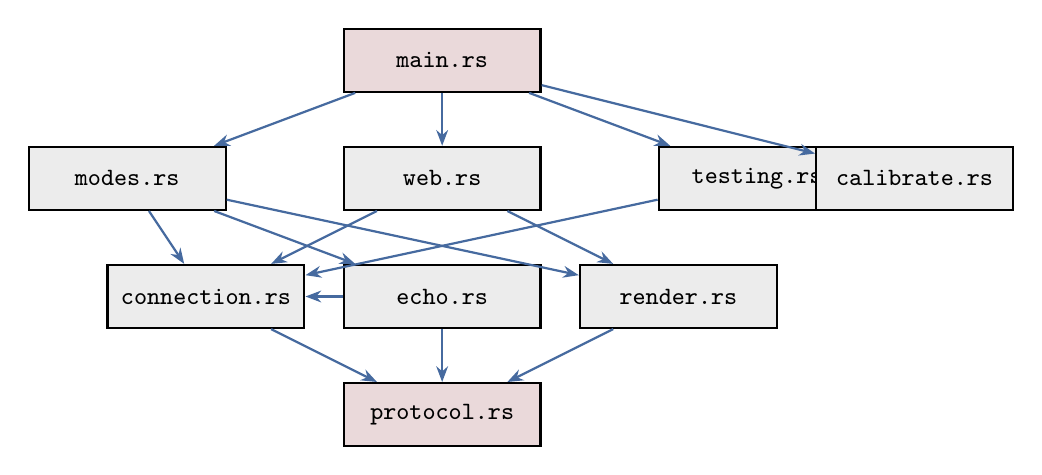
\begin{tikzpicture}[
    mod/.style={draw, thick, minimum width=2.5cm, minimum height=0.8cm, align=center, fill=black10, font=\ttfamily\small},
    dep/.style={-{Stealth[length=2mm]}, thick, color=atlantic},
]

\node[mod, fill=garnet!15] (main) at (0, 3) {main.rs};
\node[mod] (modes) at (-4, 1.5) {modes.rs};
\node[mod] (web) at (0, 1.5) {web.rs};
\node[mod] (testing) at (4, 1.5) {testing.rs};
\node[mod] (calibrate) at (6, 1.5) {calibrate.rs};
\node[mod] (connection) at (-3, 0) {connection.rs};
\node[mod] (echo) at (0, 0) {echo.rs};
\node[mod] (render) at (3, 0) {render.rs};
\node[mod, fill=garnet!15] (protocol) at (0, -1.5) {protocol.rs};

\draw[dep] (main) -- (modes);
\draw[dep] (main) -- (web);
\draw[dep] (main) -- (testing);
\draw[dep] (main) -- (calibrate);
\draw[dep] (modes) -- (connection);
\draw[dep] (modes) -- (echo);
\draw[dep] (modes) -- (render);
\draw[dep] (web) -- (connection);
\draw[dep] (web) -- (render);
\draw[dep] (testing) -- (connection);
\draw[dep] (echo) -- (protocol);
\draw[dep] (connection) -- (protocol);
\draw[dep] (render) -- (protocol);
\draw[dep] (echo) -- (connection);

\end{tikzpicture}
\caption{Module dependency graph. Shaded modules are the primary entry points.}
\label{fig:modules}
\end{figure}

\begin{description}[style=nextline, leftmargin=2cm]
\item[\texttt{main.rs}] Entry point, CLI argument parsing, IP resolution, mode dispatch.
\item[\texttt{protocol.rs}] Wire protocol implementation: constants, command builders, echo decoders, discovery, network interface detection.
\item[\texttt{connection.rs}] \texttt{RadarConnection} state machine: auth, control channel, init, TX control, keepalive, response parsing. Also provides the \texttt{create\_echo\_socket} helper.
\item[\texttt{echo.rs}] Echo packet header parsing, rotation statistics collection, CSV export.
\item[\texttt{render.rs}] PPI image rendering (spoke-to-pixel transformation, PNG encoding).
\item[\texttt{modes.rs}] CLI mode implementations: handshake, TX toggle, echo listen, full cycle, dump raw, render live/CSV, discover.
\item[\texttt{web.rs}] HTTP server (Axum), all REST API endpoints, echo listener thread, pattern execution engine.
\item[\texttt{testing.rs}] Validation suite, A/B command testing with before/after PPI captures.
\item[\texttt{calibrate.rs}] Calibration pattern generator, multi-parameter sweep runner.
\end{description}


\subsection{Connection State Machine}

The \texttt{RadarConnection} struct manages the radar lifecycle through five states.

\begin{figure}[h]
\centering
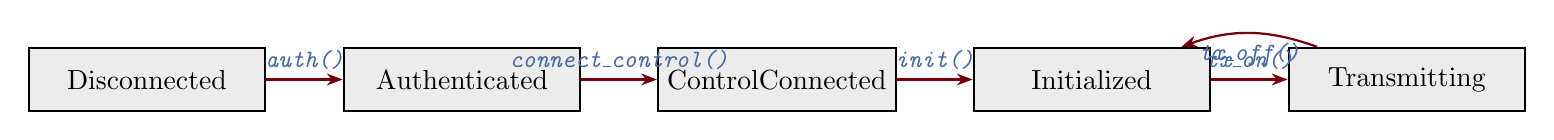
\begin{tikzpicture}[
    state/.style={draw, thick, minimum width=3cm, minimum height=0.8cm, align=center, fill=black10},
    trans/.style={-{Stealth[length=2mm]}, thick, color=garnet},
    label/.style={font=\small\itshape, color=atlantic, midway, above},
]

\node[state] (disc) at (0, 0) {Disconnected};
\node[state] (auth) at (4, 0) {Authenticated};
\node[state] (ctrl) at (8, 0) {ControlConnected};
\node[state] (init) at (12, 0) {Initialized};
\node[state] (tx) at (16, 0) {Transmitting};

\draw[trans] (disc) -- (auth) node[label] {\texttt{auth()}};
\draw[trans] (auth) -- (ctrl) node[label] {\texttt{connect\_control()}};
\draw[trans] (ctrl) -- (init) node[label] {\texttt{init()}};
\draw[trans] (init) -- (tx) node[label] {\texttt{tx\_on()}};
\draw[trans] (tx) to[bend right=20] node[font=\small\itshape, color=atlantic, midway, below] {\texttt{tx\_off()}} (init);

\end{tikzpicture}
\caption{RadarConnection state machine.}
\label{fig:state_machine}
\end{figure}

The convenience method \texttt{connect\_full()} chains \texttt{auth()} $\to$ \texttt{connect\_control()} $\to$ \texttt{init()} in sequence.


%=============================================================================
\section{Web API Reference}
%=============================================================================

The web server runs on the host at port 8080 (configurable) and provides a REST API for browser-based radar control. All endpoints return JSON or raw image data.

\subsection{Power and Connection}

\begin{longtable}{@{}llp{7cm}@{}}
\toprule
\textbf{Endpoint} & \textbf{Method} & \textbf{Description} \\
\midrule
\endhead
\texttt{/toggle\_echo} & GET & Toggle TX ON/OFF. Returns \texttt{"on"} or \texttt{"off"}. \\
\texttt{/reconnect} & GET & Reconnect to the radar (full init). Returns \texttt{"ok"} or error. \\
\bottomrule
\end{longtable}

\subsection{Radar Settings}

All settings endpoints accept parameters via query string (e.g., \texttt{/set\_range?value=6}).

\begin{longtable}{@{}llp{7cm}@{}}
\toprule
\textbf{Endpoint} & \textbf{Parameter} & \textbf{Description} \\
\midrule
\endhead
\texttt{/set\_range} & \texttt{value} (wire index) & Set radar range \\
\texttt{/set\_gain} & \texttt{value} (0--255) & Set gain level \\
\texttt{/set\_pulse\_width} & \texttt{value} (0--3) & Set pulse width \\
\texttt{/set\_bearing\_resolution} & \texttt{value} (0--3) & Set rez boost level \\
\texttt{/set\_acsea} & \texttt{value} (0--255) & Set sea clutter filter \\
\texttt{/set\_acrain} & \texttt{value} (0--255) & Set rain clutter filter \\
\texttt{/set\_near\_stc} & \texttt{value} & Set near STC \\
\texttt{/set\_middle\_stc} & \texttt{value} & Set middle STC \\
\texttt{/set\_far\_stc} & \texttt{value} & Set far STC \\
\texttt{/set\_main\_bang} & \texttt{value} & Set main bang suppression \\
\texttt{/set\_interference\_rejection} & \texttt{value} (0--1) & Toggle IR filter \\
\texttt{/set\_bird\_mode} & \texttt{value} (0--3) & Set bird mode level \\
\texttt{/set\_doppler} & \texttt{value} (0--2) & Set Doppler mode \\
\texttt{/set\_antenna\_revolution} & \texttt{value} & Set rotation speed \\
\bottomrule
\end{longtable}

\subsection{State Queries}

\begin{longtable}{@{}llp{7cm}@{}}
\toprule
\textbf{Endpoint} & \textbf{Method} & \textbf{Description} \\
\midrule
\endhead
\texttt{/get\_current} & GET & Returns JSON with current radar settings (range, gain, pulse, etc.) \\
\texttt{/get\_system\_info} & GET & Returns JSON with firmware version, connection status, TX state \\
\texttt{/system\_metrics} & GET & Returns JSON with system metrics (CPU, memory, uptime) \\
\bottomrule
\end{longtable}

\subsection{Echo Image}

\begin{longtable}{@{}llp{7cm}@{}}
\toprule
\textbf{Endpoint} & \textbf{Method} & \textbf{Description} \\
\midrule
\endhead
\texttt{/newest\_png} & GET & Returns the latest PPI image as PNG (800$\times$800 RGBA) \\
\texttt{/newest\_trail} & GET & Alias for \texttt{/newest\_png} \\
\texttt{/newest\_detection} & GET & Alias for \texttt{/newest\_png} \\
\bottomrule
\end{longtable}

\subsection{Recording}

\begin{longtable}{@{}llp{7cm}@{}}
\toprule
\textbf{Endpoint} & \textbf{Method} & \textbf{Description} \\
\midrule
\endhead
\texttt{/toggle\_recording} & GET & Start/stop echo CSV recording. Creates timestamped output directory. \\
\bottomrule
\end{longtable}

\subsection{Pattern Execution}

Pattern execution allows automated parameter sweeps for calibration and data collection.

\begin{longtable}{@{}llp{7cm}@{}}
\toprule
\textbf{Endpoint} & \textbf{Method} & \textbf{Description} \\
\midrule
\endhead
\texttt{/run\_pattern} & GET & Run a single pattern step (query params: range, gain, pulse, rezboost, speed, interp, repeat) \\
\texttt{/run\_pattern\_queue} & POST & Run a sequence of pattern steps. Body format: \texttt{repeat:base64(steps)} where steps are semicolon-separated \\
\texttt{/stop\_pattern} & GET & Stop the currently running pattern \\
\texttt{/pattern\_status} & GET & Returns \texttt{running|detail} or \texttt{idle|detail} \\
\bottomrule
\end{longtable}

Each pattern step is encoded as a comma-separated string: \texttt{range,gain,pulse,rezboost,speed,interp,repeat\_rotations}. Steps are separated by semicolons. The entire step string is base64-encoded in the POST body.


%=============================================================================
\section{CLI Modes}
%=============================================================================

The \texttt{radar-client} binary supports multiple operating modes selected by the first positional argument.

\begin{lstlisting}
radar-client [--radar-ip IP] [--host-ip IP] <mode> [args...]
\end{lstlisting}

\begin{longtable}{@{}lp{9cm}@{}}
\toprule
\textbf{Mode} & \textbf{Description} \\
\midrule
\endhead
\texttt{handshake} & Perform full authentication and initialization. Print firmware info and register values. \\
\texttt{tx-on} & Initialize and enable transmitter. \\
\texttt{tx-off} & Initialize and disable transmitter. \\
\texttt{echo} & Listen for multicast echo packets without authentication (passive monitoring). \\
\texttt{full} & Full cycle: init, TX ON, collect one rotation of echo data, TX OFF. \\
\texttt{command} & Send test commands and display acknowledgments. \\
\texttt{render-csv \textit{file} [\textit{out}]} & Render a previously recorded CSV file as a PPI image (offline, no radar needed). \\
\texttt{render-live [\textit{out}]} & Capture one rotation and render to PNG. \\
\texttt{dump-raw [\textit{count}]} & Dump raw echo packet headers and hex data. \\
\texttt{test-commands} & A/B command verification with before/after PPI captures. \\
\texttt{calibrate \textit{args}} & Run calibration pattern sweeps with configurable parameter ranges. \\
\texttt{discover} & Broadcast discovery beacons and listen for radar responses. \\
\texttt{validate} & Run the comprehensive 6-phase validation suite. \\
\texttt{web [\textit{port}] [\textit{webdir}]} & Start the HTTP server (default port 8080, web files from \texttt{../web}). \\
\bottomrule
\end{longtable}


%=============================================================================
\section{Testing and Validation}
%=============================================================================

The project includes 27 integration tests that require a live radar connection. Tests must be run sequentially since the radar only supports one active control connection.

\begin{lstlisting}
cargo test -- --test-threads=1
\end{lstlisting}

\subsection{Test Categories}

\subsubsection{Connection Tests (6)}

These tests verify the fundamental communication path: TCP authentication, control channel establishment, full initialization, firmware version retrieval, keepalive exchange, and multicast echo socket creation.

\subsubsection{TX Tests (3)}

These tests verify transmitter control: TX ON/OFF cycling, echo packet reception after TX ON, and full rotation data collection (8{,}192 spokes).

\subsubsection{Settings Tests (14)}

Each test follows a set-and-read pattern: send a \texttt{\$S} command to change a parameter, then send the corresponding \texttt{\$R} query to verify the change was accepted. Covers range, manual gain, auto gain, pulse width, rez boost, sea clutter, rain clutter, near/middle/far STC, main bang suppression, interference rejection, bird mode, Doppler, and antenna revolution speed.

\subsubsection{Echo Impact Tests (2)}

These tests verify that parameter changes produce measurable effects in the echo data. One test compares echo amplitudes at different gain levels; the other verifies that range changes produce different data patterns. These tests require physical targets in the radar's field of view to produce reliable results.

\subsubsection{Render Integration Test (1)}

Captures a full rotation of live echo data and renders it to a PNG file, verifying the complete pipeline from UDP multicast reception through spoke decoding to PPI image generation.


%=============================================================================
\section{Calibration System}
%=============================================================================

The calibration system enables automated parameter sweeps for systematic data collection. A calibration pattern defines a sequence of radar configurations, each held for a specified number of antenna rotations.

\subsection{Pattern Step Definition}

Each step specifies seven parameters.

\begin{lstlisting}
ControlStep {
    range:          u16,    // wire index (0-21)
    gain:           u16,    // 0-255
    pulse_length:   u16,    // 0-3
    rez_boost:      u16,    // 0-3
    rotation_speed: u16,    // antenna speed mode
    interpolation:  u16,    // spoke interpolation target
    repeat:         u16,    // rotations to hold this config
}
\end{lstlisting}

\subsection{Differential Command Generation}

When transitioning between pattern steps, only the parameters that changed are sent to the radar. This minimizes control channel traffic and avoids unnecessary state transitions.

\subsection{Pattern Generation}

The \texttt{generate\_pattern} function creates a full combinatorial sweep across multiple parameter ranges, producing all possible combinations of the specified values for systematic characterization.


%=============================================================================
\section{Proprietary Library Reference}
%=============================================================================

The original Furuno \texttt{libNAVNETDLL.so} shared library was reverse-engineered to develop this implementation. Table~\ref{tab:symbols} summarizes the library's module structure. The full symbol classification (6{,}102 defined functions) is available in \texttt{protocol-notes/symbols.md}.

\begin{table}[h]
\centering
\caption{libNAVNETDLL.so module breakdown.}
\label{tab:symbols}
\begin{tabular}{@{}llrl@{}}
\toprule
\textbf{Module} & \textbf{Prefix} & \textbf{Count} & \textbf{Relevance} \\
\midrule
Radar Command Set & \texttt{RmcSet*} & 154 & Reimplemented \\
Radar Command Get & \texttt{RmcGet*} & 143 & Reimplemented \\
Radar Command Req & \texttt{RmcReq*} & 133 & Reimplemented \\
Radar Module & \texttt{Rm*} & 67 & Reimplemented \\
NAVNET Common & \texttt{Nc*} & 310 & Reimplemented \\
ARPA & \texttt{Rma*} & 13 & Not yet \\
Echo Sounder & \texttt{Esc*/Es*} & 882 & Not applicable \\
FNET Network & \texttt{nn*} & 188 & Internal \\
Licensing & \texttt{Flm*} & 46 & Bypassed \\
Crypto & \texttt{Blowfish*/bf*} & 14 & Not needed \\
\bottomrule
\end{tabular}
\end{table}


\end{document}
